\chapter{Impact of Recirculation in Dynamic Contrast-Enhanced Ultrasound: a Simulation Study}\label{chapter:IRBM}
% \usepackage{amsmath,units,stmaryrd}
% \usepackage{textgreek,graphicx,booktabs,multirow,xcolor,placeins}

\section{Abstract}
\textit{Objectives} The impact of recirculation on the quantification of perfusion is often neglected. It can however introduce a bias or some variability in the estimation of perfusion parameters and thus hamper comparison between exams.
\textit{Methods} Time-intensity curves (TICs) were simulated using a one-compartment model fed by an arterial input function (AIF). A simple model was developed to simulate recirculation in the AIF. Using AIF with and without recirculation, and sets of regional perfusion parameters, TICs corresponding to different tissue regions were simulated by convolution of the AIFs with the transfer function associated to each region. 150 simulations for each of the 10 noise levels were then computed. For each simulated study, six quantification methods based on either Log-Normal modeling or relative compartmental modeling were tested. Variations of the conventional Log-Normal model were also investigated, including using parameters estimated in a reference tissue for normalization purposes, and fitting only the first phase of the TIC to avoid recirculation. \textit{Results} The impact of recirculation varies according to the quantification method. Restricting parameter estimation to the first samples of the TICs, before recirculation occurs, appears to be the worst strategy. Errors are largely minimized when using a reference tissue to establish relative parameters. The most robust approach is the compartmental modeling based on a reference tissue and applied to multiple regions with a regularization constraint. 
\textit{Conclusion} This simulation study demonstrates the influence of recirculation on the estimation of perfusion parameters. To reduce the impact of this unavoidable effect, the quantification method based on compartmental modeling and using a reference tissue appear to be the most reliable strategy.


\section{Introduction}
\label{sec:intro}

With the advent of contrast agents, perfusion imaging has been developed for different medical imaging modalities, including PET, CT, MRI, and more recently ultrasound. Perfusion parameters including regional tissue blood volume and tissue blood flow are functional indices which can help in the  diagnosis of some vascular abnormalities, such as ischemia. Vascular modification in tumors is also a key application of perfusion imaging and can be used in order to assess tumor diagnosis or tumor monitoring~\cite{Dietrich:2012kw}. 

A widely used approach to estimate perfusion parameters relies on bolus injections of contrast agent and dynamic recording of frames. However the quantification of signal and the estimation of perfusion parameters through mathematical modeling remains a hard task and has generated a lot of research work~\cite{Turco:2016}. An accurate and robust estimation of perfusion parameters is of course crucial to compare perfusion imaging exams meaningfully. This is primordial in order to allow inter-subject exams or to perform monitoring. 
Among the different mathematical models that have been proposed in contrast-enhanced ultrasound (CEUS) studies, little attention has been devoted to compartmental modeling, despite its wide use in PET or MRI studies. Indeed, explicit modeling using for instance a Log-Normal function is often recommended to analyze dynamic data~\cite{Strouthos2010it,Dietrich:2012kw}.
Of course different reasons can explain this restricted use of the comparmental approach; among them the difficulty in estimating a correct arterial input function in dynamic ultrasound images can be cited. To get rid of this difficulty which occurs also while using other imaging techniques, some authors in PET imaging and more recently in MRI have proposed to use a reference tissue in order to define relative perfusion parameters~\cite{Yankeelov2005de,CardenasRodriguez2013em}, defined as the ratio between the perfusion parameters in the tissue of interest and the perfusion parameters defined in the reference tissue. Our group has recently shown the practical interest of this approach in a test-retest protocol applied to a murine tumor model~\cite{Doury2016fi,Doury2017wn}. 

As no absolute gold-standard exist for preclinical or clinical studies, simulations can be used to assess the performance of different models and compare them. Of course, as it is quite complex to reproduce in silico the complexity of in vivo, the extrapolation of simulations to real cases should be done very carefully. However they can be used to focus on one specific trait and to quantify its impact. In the present study, the studied trait was recirculation, since this process is often overlooked when quantifying CEUS exams. This is especially true in small animals, where recirculation occurs quickly and can overlap with the first pass of the bolus of micro-bubbles in tissues, affecting the time-intensity curves (TICs) used for quantification.

For the present study, a one-compartmental model was assumed to be representative of the underlying physiology that is observable at a regional scale. Different values of perfusion parameters (tissue blood flow, tissue blood volume and time-delays) were simulated in order to better apprehend the spatial heterogeneity that can be observed inside a tumor. The values of these parameters were derived from results obtained in a preclinical study in order to be coherent with practical observations. In addition to recirculation, the impact of signal to noise ratio was  studied. For the modelling apporach, two versions of the Log-Normal model (absolute and relative), and two versions of the relative one-compartment model (one based on a single region, one taking advantage from the existence of multiple regions) were considered. In addition, in order to limit the impact of recirculation while estimating perfusion parameters with the Log-Normal model, a simple and popular strategy was tested which consists in using the first samples of TICs, i.e.~samples acquired before recirculation occurs~\cite{Lowerison2017}. These six perfusion quantification methods were fitted to simulated TICs to study the precision and  the accuracy of the estimated perfusion parameters. 

\section{Theory}

\subsection{One-compartment vascular model}
\label{sec:simmdl}
Consider $N$ vascularized tissue regions $T_i$, $i=1,..,N$ in a spatial domain, each region being an homogeneous compartment fed by the same arterial input function (AIF), $C_A$. This mono-compartmental hypothesis is realistic since the distribution of microbubbles is restricted to the vascular space~\cite{Gunn2001cx}. Each tissue TIC, $C_{T_i}$, is characterized by a tissue blood volume $V_i$, and a tissue blood flow $F_i$. Since introducing a time-delay parameter in this model was shown to improve the quality of fit in tumor tissues~\cite{Doury2017wn}, a parameter $D_i$ reflecting the transit time of the contrast agent from the feeding artery to the tissue was also considered. 
The mathematical relationship between the tissue TIC and the TIC in its feeding artery is given by equation \ref{eq:CM}:
\begin{equation}
 C_{T_i} = C_A \ast h_{F_i,V_i,D_i}
\label{eq:CM}
\end{equation}
where $h_{F_i,V_i,D_i} (t) = F_i \cdot \mathrm{e}^{-\frac{F_i}{V_i} \left( t - D_i \right)}\forall t \leq D_i, 0$ else, represents the transfer function of the $i^{th}$ tissue region.

\subsection{Simplified recirculation model}
After injection in a vein, the bolus of microbubbles travels through the lungs and heart chambers before being distributed in the whole body through the arterial system. After this first pass in the tissues, microbubbles return to the venous system for another circulation loop. During each loop, the bolus is attenuated by the natural disruption of microbubbles, and their filtration through the lungs and the liver. Additionally, the bolus length spreads in time because of the inhomogeneous path length of the individual microbubbles~\cite{Blomley1997ff}.

An AIF with recirculation, $C_{Aw}$, can therefore be approximated by a sum of consecutive passes of the bolus in the region of interest (equation \ref{eq:RC}): 
\begin{equation}
\label{eq:RC}
C_{Aw} \left(t\right) = C_{A1}(t) + \sum_{r=1}^{N_R} R_r \left(t\right),
\end{equation}
where $C_{A1}(t)$ is the TIC of the first pass of the bolus, $R_r(t)$ is the TIC of the r$^{\mathrm{th}}$ recirculation, and $N_R$ is the number of recirculation loops which are taken into account. The TIC, $C_{A1}(t)$, thus represents the AIF without recirculation.

To go further in the simulation process, a simplified recirculation model was defined, assuming a constant recirculation period $\gamma$, a constant recirculation fraction $\beta$ (the fraction of microbubbles remaining from the previous bolus pass taking into account bubble disruption and filtration), a constant spread factor $\alpha$ through the different recirculation loops, and an exponential spread and decay of the signal. The r$^{\mathrm{th}}$ recirculation TIC, $R_r(t)$, was simulated by equation \ref{eq:Rn}:
\begin{equation}
R_r \left( t - r \gamma \right) = \frac{\beta^r}{\alpha^r} C_{A1} \left( \frac{t }{\alpha^r} \right)
\label{eq:Rn}
\end{equation}
Examples of AIF with and without recirculation are shown in Figure~\ref{fig:recmod} (first row). For the present study, $C_{A1}(t)$ is represented by a log-normal function, $C_{Aw}(t)$ is computed using $\alpha = 2$, $\beta = 30\%$, $\gamma = 20$~s and $N_R=7$. TICs were simulated for a total duration of $165$~s with a frame rate of 3~Hz.

\begin{figure}
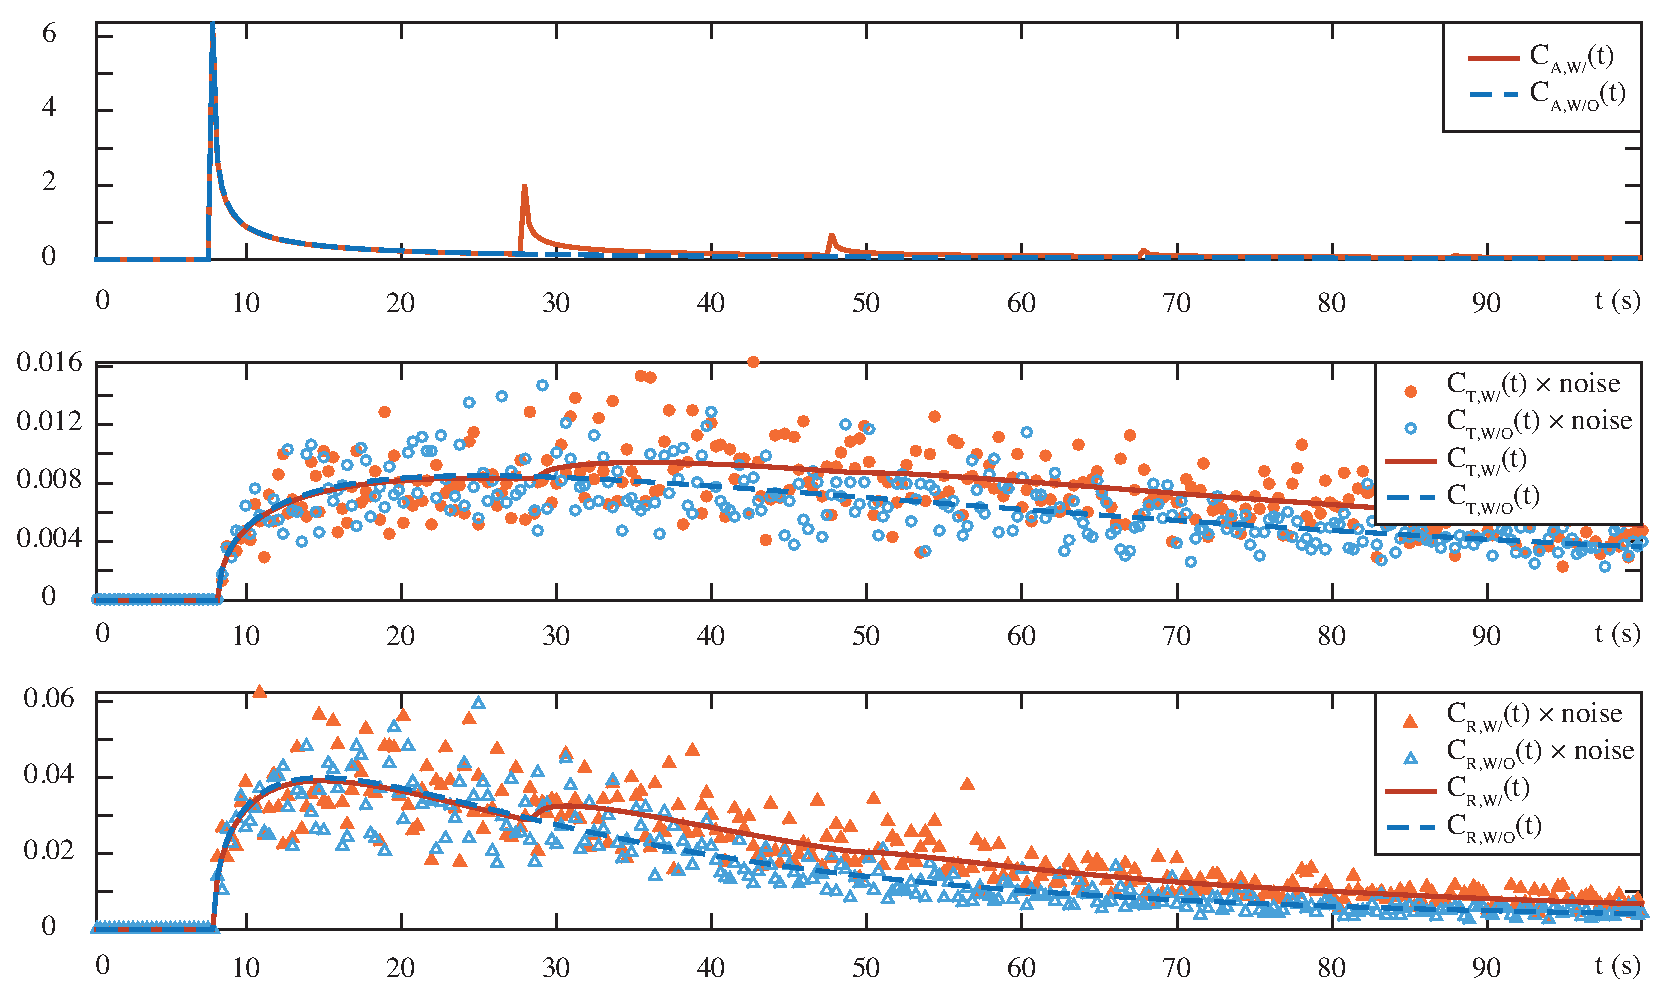
\includegraphics[width=\linewidth]{Ch5_simRC_CaCt4Cr.eps}
\vspace{-5mm}
\caption{Simulated TICs with (orange) and without recirculation (blue) corresponding to noise-free AIF (top), examples of noise-free and noisy TICs in the fourth tissue region (middle) and in the reference tissue (bottom). The first hundred seconds are displayed here.}
\label{fig:recmod}
\vspace{-3mm}
\end{figure}

\subsection{Noise model}
A multiplicative noise model following a gamma distribution~\cite{Barrois2013} while constraining the mean intensity to be 1 (unit mean). Indeed, a unit mean distribution for a multiplicative noise is the equivalent of a zero-centered distribution for additive noise. A gamma distribution is defined by two parameters: its shape parameter $\kappa$, and its scale parameter $\theta$. Enforcing a unit mean is equivalent to set $\theta = \nicefrac{1}{\kappa}$, the noise distribution $p\left(v\right)$ is then defined by Eq.~\ref{eq:Noise}:
\begin{equation}
p\left(v\right) = \nicefrac{1}{\Gamma\left(\kappa\right)} ~ \kappa^\kappa ~ v^{\kappa-1} ~ \mathrm e^{-v\kappa}, \forall~v \geq 0.
\label{eq:Noise}
\end{equation}
The parameter $\kappa$ controls the sharpness of the noise distribution, and is related to the standard deviation of the noise ditribution by $\sigma = \nicefrac{1}{\sqrt{\kappa}}$.

\subsection{Perfusion quantification methods}
\label{sec:Models}
Six perfusion quantification methods ($M_1-M_6$) were tested and compared. Among them, four relative approaches ($M_3-M_6$) making use of an in-plane reference tissue (R) were proposed to make parameters more robust to inter-exam changes (due to unavoidable experimental or physiological varying conditions). Furthermore, the last method ($M_6$) takes advantage of the multiple regions that can be defined inside an image.

\subsubsection{Methods $M_1$ and $M_2$ - Log-Normal model (LN)}
The Log-normal function is an explicit model that depends on four parameters, it is frequently used to fit TICs, in particular from dynamic contrast-enhanced ultrasound studies~\cite{Strouthos2010it}.
From this model, the area under the curve $AUC_i$, which is proportional to the tissue blood volume (see Appendix for proof) and $\tau_i$ a time parameter reflecting the delay between the beginning of the acquisition and the arrival of the first microbubbles in the tissue of interest are directly estimated. In addition, the wash-in rate ($WIR_i$), that is the maximal slope of the uptake part of the TIC, a parameter related to the tissue blood flow (see Appendix for proof), is commonly derived. Appendix shows the analytical expression of the $AUC$ and $WIR$ parameters, using the conventional expression of the Log-Normal model.
For the first method ($M_1$), all the time samples are analyzed while for the second model ($M_2$), the analysis is restricted to the first pass of the bolus, which roughly corresponds to the wash-in phase.

\subsubsection{Methods $M_3$ and $M_4$ - relative Log-Normal model (rLN)}
The relative Log-Normal models propose the comparison of the LN model parameters estimated in the tissue region $i$ ($AUC_i$, $WIR_i$, and $\tau_i$) with the corresponding values estimated in the reference tissue $R$ ($AUC_R$, $WIR_R$, and $\tau_R$), following equation \ref{eq:LNr}:
 \begin{equation}
 rAUC_i = \frac {AUC_i} {AUC_R}, rWIR_i = \frac {WIR_i} {WIR_R}, \Delta = \tau_i - \tau_{R}.
 \label{eq:LNr}
\end{equation}
For the method $M_3$, all the time samples are analyzed while for the method $M_4$, the analysis is restricted to the first pass of the bolus.

\subsubsection{Methods $M_5$ - relative one-compartment model (rLin)}
The model M5 is derived from the one-compartment model presented in Section~\ref{sec:simmdl}. It was proposed to take into account the multiple cases for which the estimation of the AIF is tricky, see for instance~\cite{Doury2017wn}.
It assumes that the tissue region and the reference tissue are parallel single compartments, fed by a common AIF. 
Writing equation~(\ref{eq:CM}) respectively for $C_{T_i}$ and $C_R$, and rearranging them, a convolution equation that is independent of the AIF can be deduced. Four related perfusion parameters~\cite{Doury2017wn}, defined by Eq.~\ref{eq:rLin}, can then be estimated as a linear function:
\begin{equation}
rF_i = F_i/F_R, rV_i = V_i/V_R, k_i = F_i/V_i, \delta_i = D_i - D_R.
\label{eq:rLin}
\end{equation}
When the time delay $\delta_i$ is estimated (defined as the inflexion point after temporal filtering), the convolution equation can be written as follows:
\begin{equation}
W_i(t)= rF_i \cdot X(t) + rV_i \cdot k_i \cdot Y(t) - k_i \cdot Z_i(t), \forall t \geq \delta_i.
\label{eq:rLin2}
\end{equation} 
 with $W_i(t)$~=~$C_{T_i}(t-\delta_i)$, $X(t)$~=~$C_R(t-\delta_R)$, $Y(t)$~=~$\int_0^t C_R \left(\tau-\delta_R\right)\mathrm d\tau$,
and $Z_i(t)$~=~$\int_0^t C_{T_i} \left(\tau-\delta_i \right)\mathrm d\tau$.
The three parameters $rF_i$, $rV_i$, and $k_i$ can thus be estimated using a linear regression which minimizes the least-squares error. For that reason the method $M_5$ is noted rLin. It was introduced in~\cite{Doury2016fi} following Patlak's approach~\cite{Patlak:1983id}.

\subsubsection{Method $M_6$ - Regularized relative one compartment model (rReg)}
This approach was proposed in~\cite{Doury2016fi} to overcome the limitations of the rLin model when it is applied to $N$ ($N$ being more than one) tissue regions. Indeed, the estimation of $N$ values of $rF_i$, $rV_i$, and $k_i$ provides $N$ potentially different values of $k_R = F_R/V_R$, since $k_R = \frac{F_R}{F_T^i}\frac{F_T^i}{V_T^i}\frac{V_T^i}{V_R} = \frac{rV_i.k_i}{rF_i}$.
The discrepancy of the values of $k_R$ can be overcome by forcing this parameter to have the same value across the different regions, i.e.~forcing a common ratio between $rV^i.k^i_T$ and $rF^i$ across all tissue regions. In summary, an iterative estimation method was proposed, each iteration being conducted in two steps : first a value for $k_R$=$\frac{rV_i.k_i}{rF_i}$ is chosen, then the $3N$ values $rF_i$, $rV_i$, and $k_i$ are estimated by applying $N$ linear optimization processes under constraints, this two-step procedure being repeated in order to minimize a global error term defined as the sum of the $N$ errors of the $N$ fittings.
As compartmental approaches take into account recirculation inherently, the  truncature approach defined for Log-Normal based models was not tested for models $M_5$ and $M_6$. 

\section{Experimental design}

\subsection{Simulations}
Simulations were derived from the small animal experiments described in~\cite{Doury2017wn}. For that study, the tumor area was divided into $32$ regions ($N=32$) and a reference tissue were considered, yielding $33$ TICs. For the present study, two sets of 33 TICs were generated, using two different arterial input functions: $C_{A1}(t)$, based on a log-normal model, and $C_{Aw}(t)$, directly derived from $C_{A1}(t)$ according to equation~(\ref{eq:RC}) to simulate recirculation (Figure~\ref{fig:recmod}).
Reference perfusion parameters $F_i$, $V_i$, $D_i$, $V_R$, $F_R$, and $D_R$, displayed on Figure~\ref{fig:simpar}, were chosen according to values estimated on an experimental dataset. The ($N+1$) TICs $C_{T_i}$ and $C_R(t)$ were simply derived using equations~(\ref{eq:CM}) and~(\ref{eq:Noise}). Fig.~\ref{fig:recmod} shows two examples of such simulated TICs.
For each configuration (without and with recirculation), noise-free and noisy TICs were simulated (see Figure~\ref{fig:recmod}. Ten noise levels with $\sigma$ varying from $0.05$ to $0.5$ were defined and in each case, 150 realizations were considered.
A Log-Normal model was fitted to each simulated noise-free $C_{T_i}$ TIC (generated using $C_{A1}(t)$), yielding reference values for $AUC_i$, $WIR_i$ and $\tau_i$. 

\begin{figure}
\center
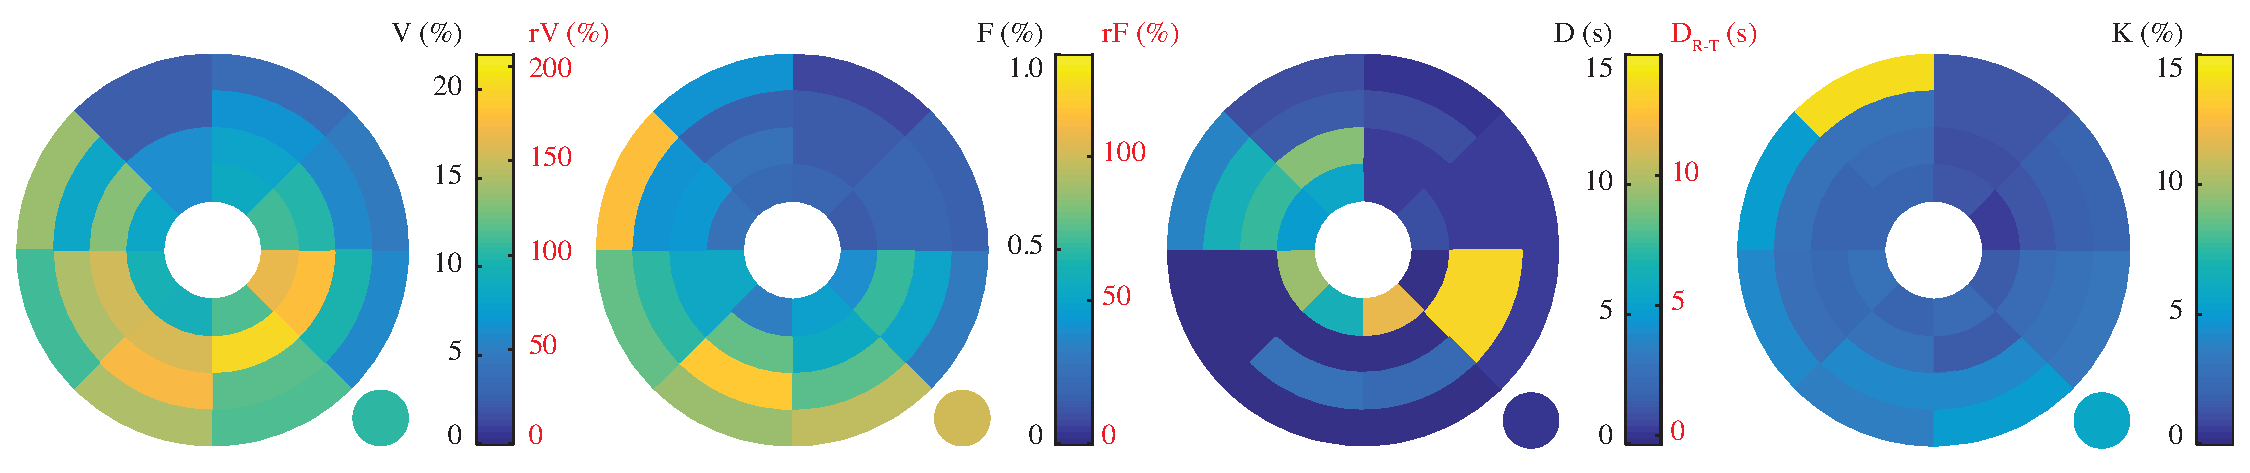
\includegraphics[width=\linewidth]{Ch5_SimRC_SimulationBullseyes.eps}
\caption{Bull's-eyes representation of the perfusion parameters used to simulate the 32 regional TICs, $C_{T_i}$ (large circle), and the reference TIC, $C_R$ (bottom right disk). From left to right: tissue blood volume ($V$), tissue blood flow ($F$), time-delay ($D$), and rate constant ($k$). The scale displayed in red color shows relative parameters: $rV$, $rF$, $\delta$ as defined by Eq.~(\ref{eq:rLin}).}
\label{fig:simpar}
\vspace{-3mm}
\end{figure}

\subsection{Data analysis}
\label{sec:datana}

For each simulated TIC $C_{hi}^{nj}(t)$, associated with configuration $h$ (for $h=1$, the AIF is $C_{A1}(t)$, for $h=2$ the AIF is $C_{Aw}(t)$), region $i$ ($i=1,..., 32$), noise level $n$ ($n=0, ...,10$) and realization $j$ ($j=1,...,150$), the different perfusion parameters $\Theta_{hi}^{nj}(M_m)$ were estimated using the six methods ($M_m$, $m=1, ..., 6$) presented in Section~\ref{sec:Models}.
As the methods $M_2$ and $M_4$ were defined to be less sensitive to recirculation, the LN model was fitted to the 20 first seconds following the time-delay estimated for each TIC, since $\gamma = 20$ seconds was the recirculation period used for simulation.

For parameters related to the tissue blood flow or to the tissue blood volume, the relative estimation error, expressed in \%, was defined as follows: 
\begin{equation}
E_{hi}^{nj}(M_m) = \frac{\Theta_{hi}^{nj}(M_m) - \Lambda_{i}(M_m)}{\Lambda_{i}(M_m)}
\end{equation}
where $\Lambda_{i}(M_m)$ is the reference value of the perfusion parameter estimated in the $i^{th}$ tissue region using method $M_m$.
For time-delay parameters the absolute estimation error was defined in seconds as: 
\begin{equation}
E_{hi}^{nj}(M_m) =\Theta_{hi}^{nj}(M_m) - \Lambda_{i}(M_m),
\end{equation}

\section{Results}
Fig.~\ref{fig:estpar4} shows statistical results related to the perfusion parameters estimated inside one specific region ($i=4$) using the six models $(M_m)$ described in section~\ref{sec:Models}, $\Theta_{h4}^{n}(M_m)$.
Indeed, the simulated values $\Lambda_{4}(M_m)$ and the median, first, and third quartile values over the 150 simulations of parameters are represented as a function of the noise level (indice $n$, proxied by $\sigma$). These results are displayed for simulations without ($h=1$) and with recirculation ($h=2$).

In complement to Fig.~\ref{fig:estpar4}, Fig.~\ref{fig:be-LN}, \ref{fig:be-rLN}, and \ref{fig:be-rLinReg} display bull's-eye representations of the median estimation errors in the 32 regions for an intermediate noise level ($\sigma=0.25, n=6$), $E_{hi}^{6}(M_m)$, for the six quantification methods and the two conditions of recirculation. 
\begin{figure}
\center
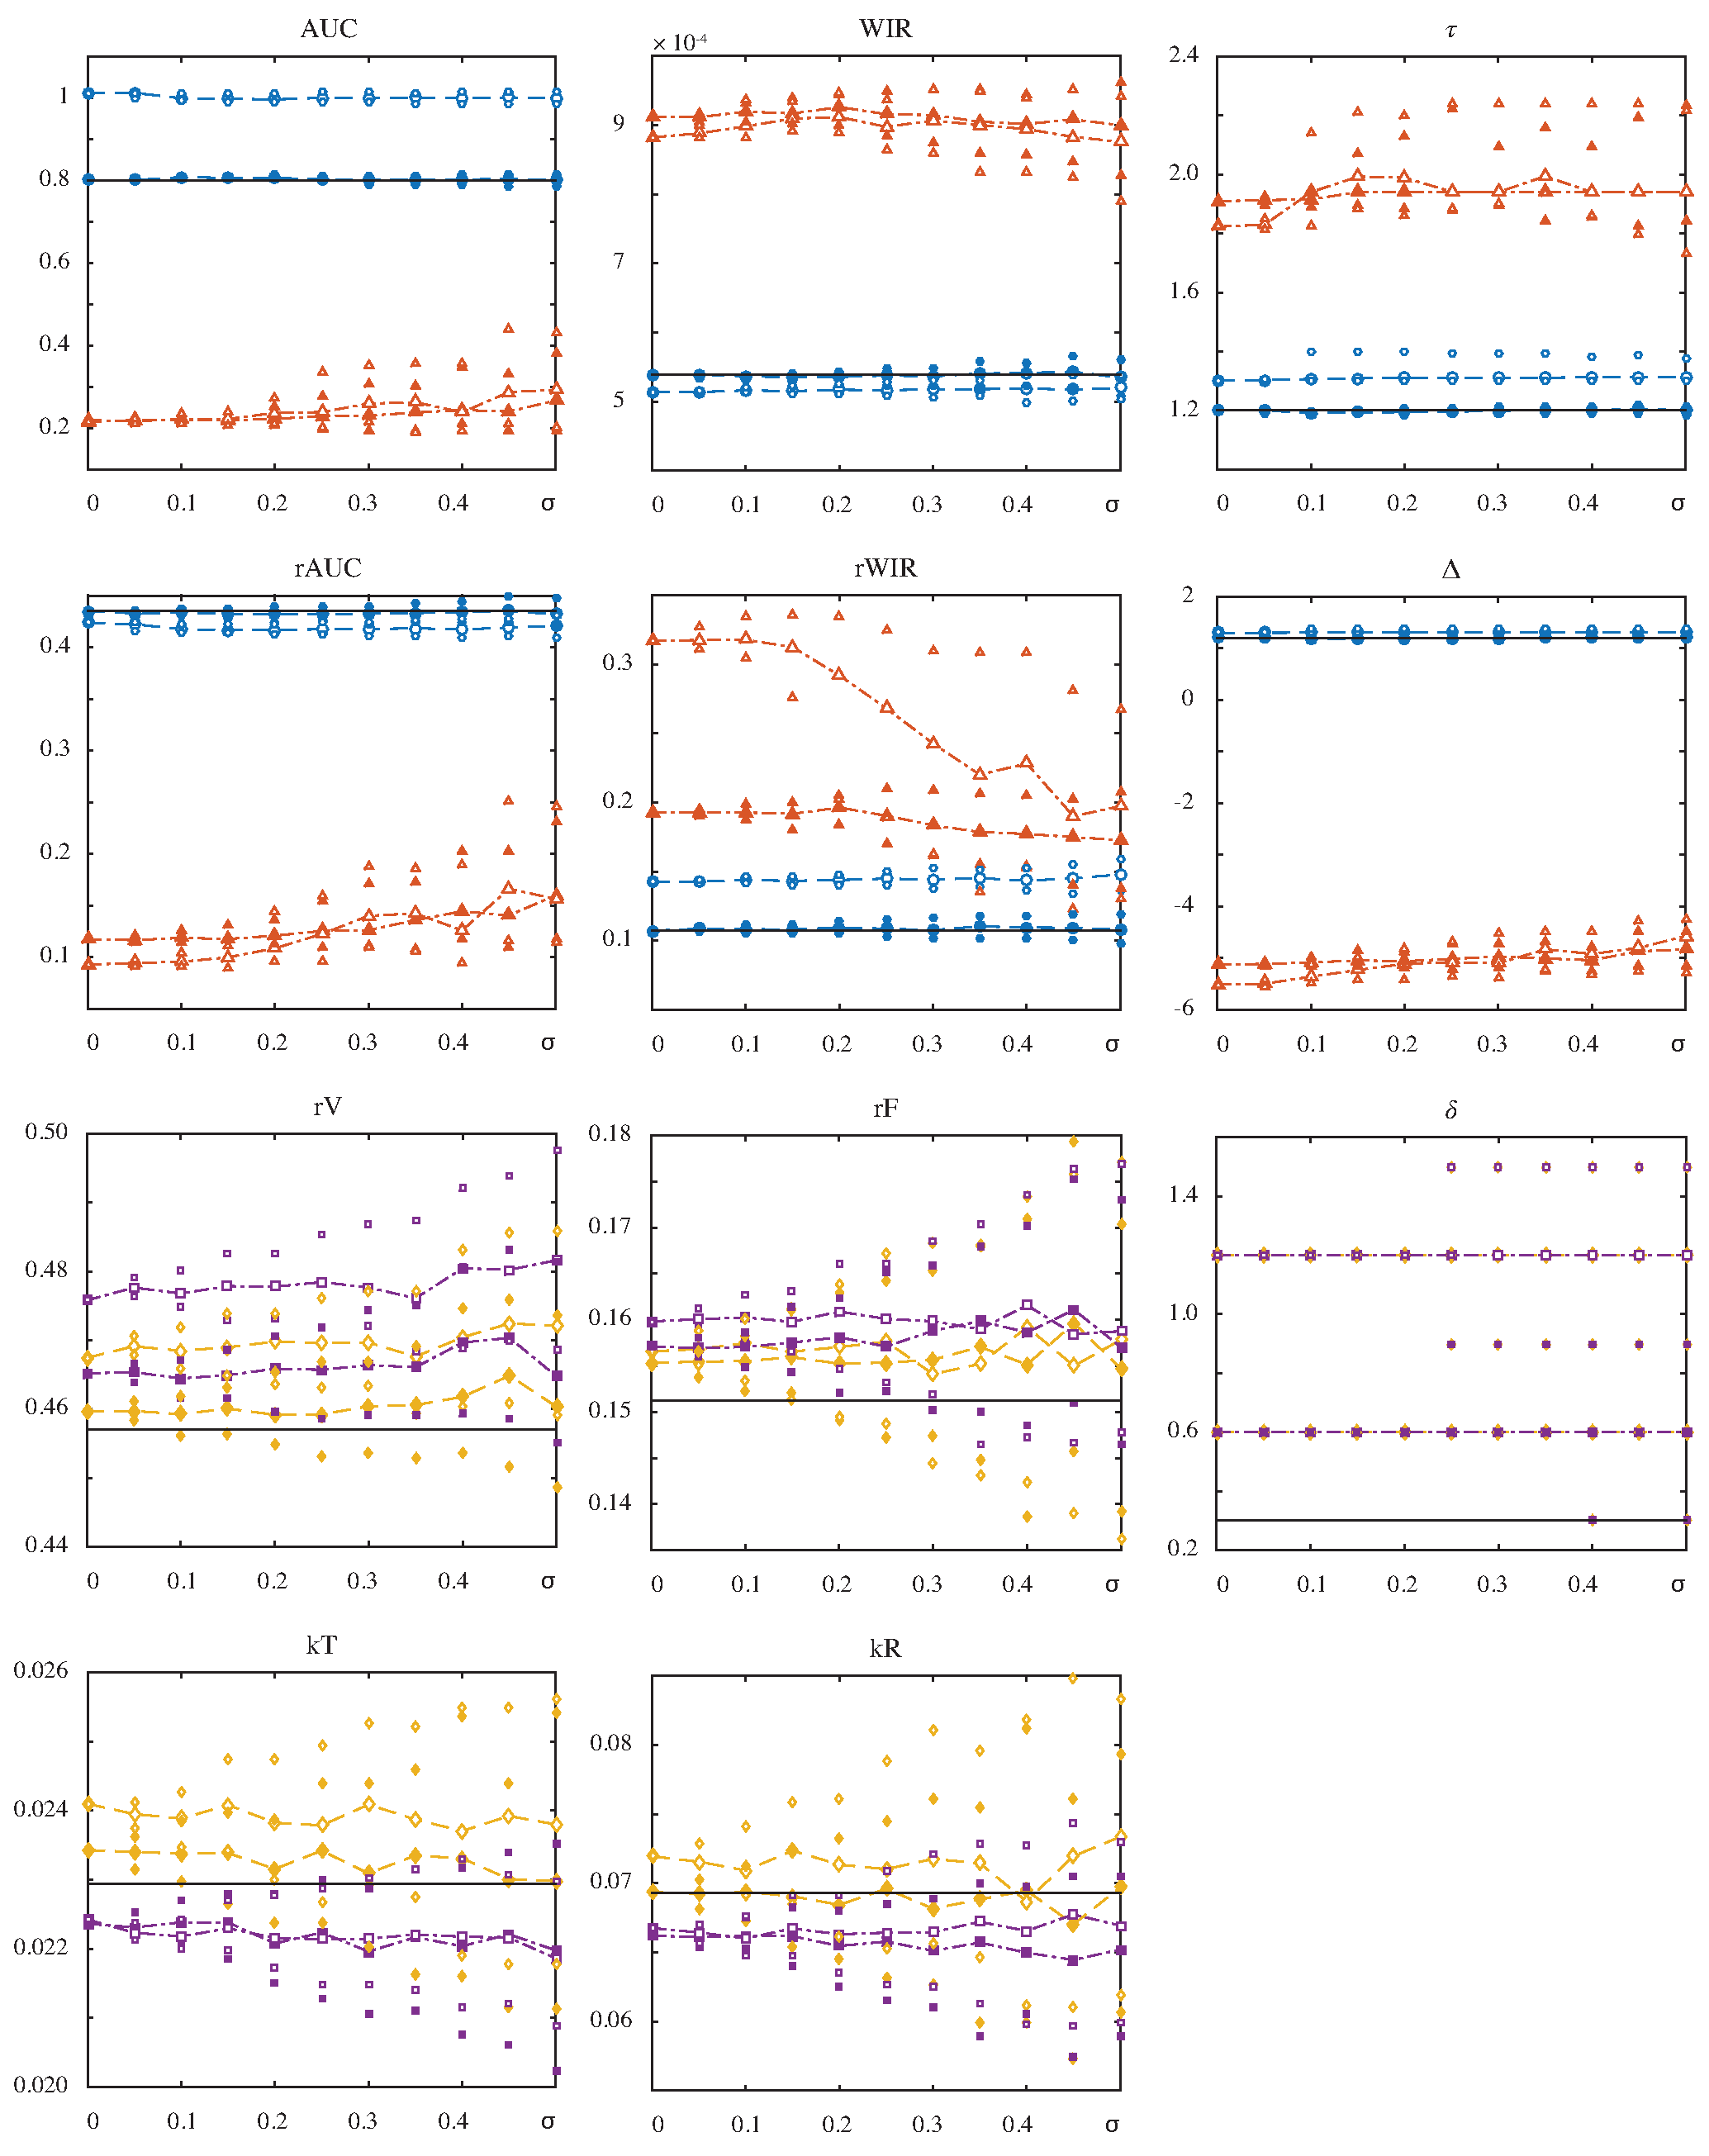
\includegraphics[width=\linewidth]{Ch5_ParamBoard_Ct4.eps}
\caption{Median values (large symbols), first and third quartiles (small symbols) of parameters estimated for the fourth tissue region $C_{T_4}$ (outer ring, upper halve, right octant). First column: tissue blood volume related parameters, second column: tissue blood flow related parameters, third column: time-delay related parameters, fourth row: rate constants in the tissue region and reference tissue. Constant lines in black represent simulated values, blue lines the estimation corresponding to the LN model, red lines the estimation corresponding to the LN model restricted to wash-in phase. Yellow color stands for rLin model, while purple color stands for rReg model. For all of the cases, filled symbols correspond to the configuration without recirculation, while empty symbols correspond to the configuration with recirculation.}
\label{fig:estpar4}
\vspace{-3mm}
\end{figure}

\begin{figure}
\center
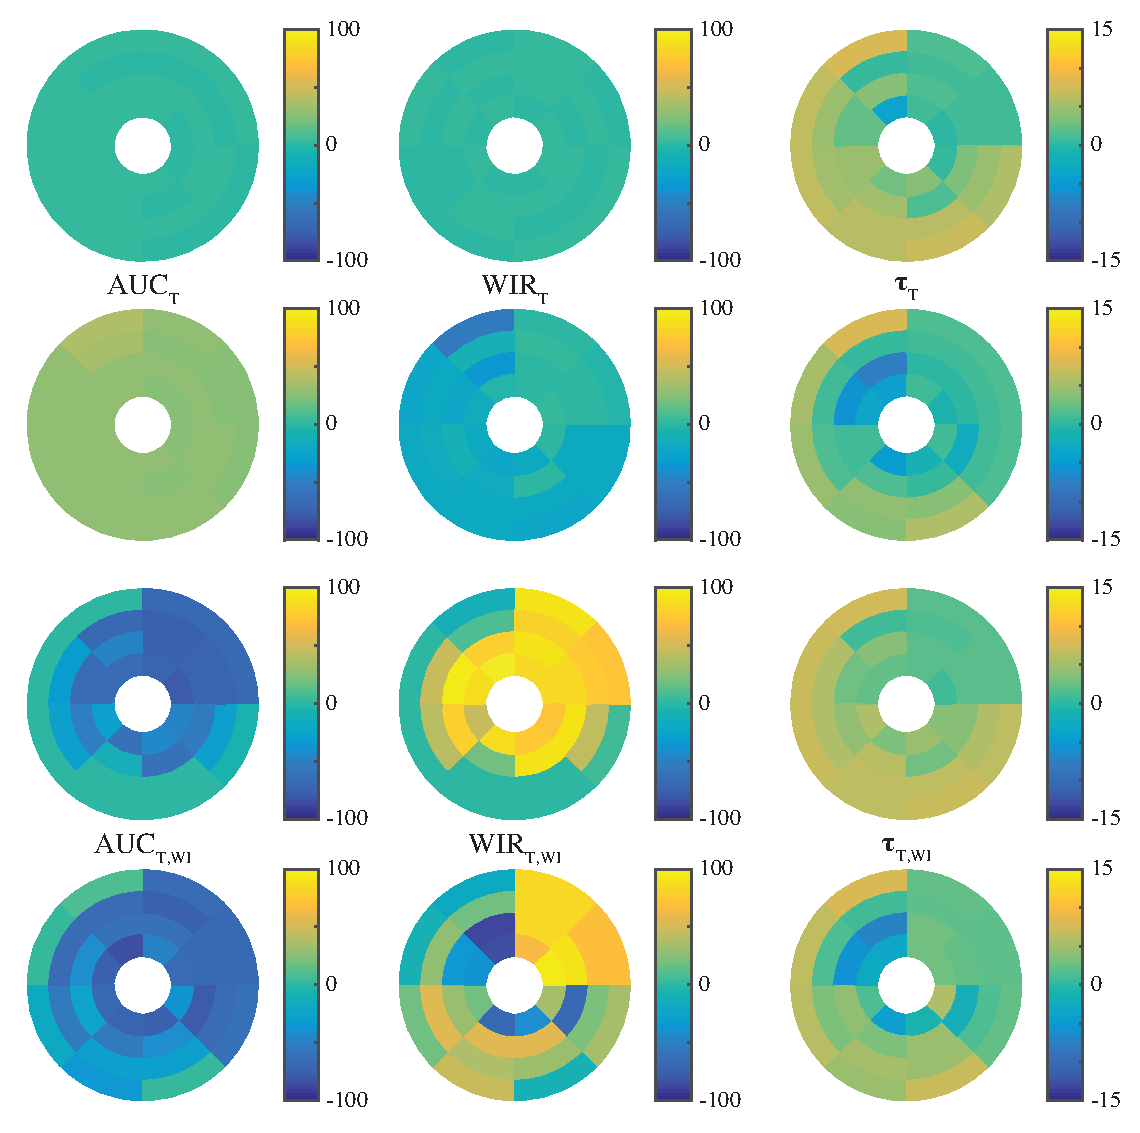
\includegraphics[width=\linewidth]{Ch5_simRC_bullseye_LN_LNwi.eps}
\caption{Bull's-eyes of the median estimation errors obtained by the LN model at the intermediate noise level. From left to right: estimation errors corresponding to tissue blood volume, tissue blood flow, time delay. From top to bottom: $M_1$ without recirculation, $M_1$ with recirculation, $M_2$ without recirculation, $M_2$ with recirculation.}
\label{fig:be-LN}
\vspace{-3mm}
\end{figure}

\begin{figure}
\center
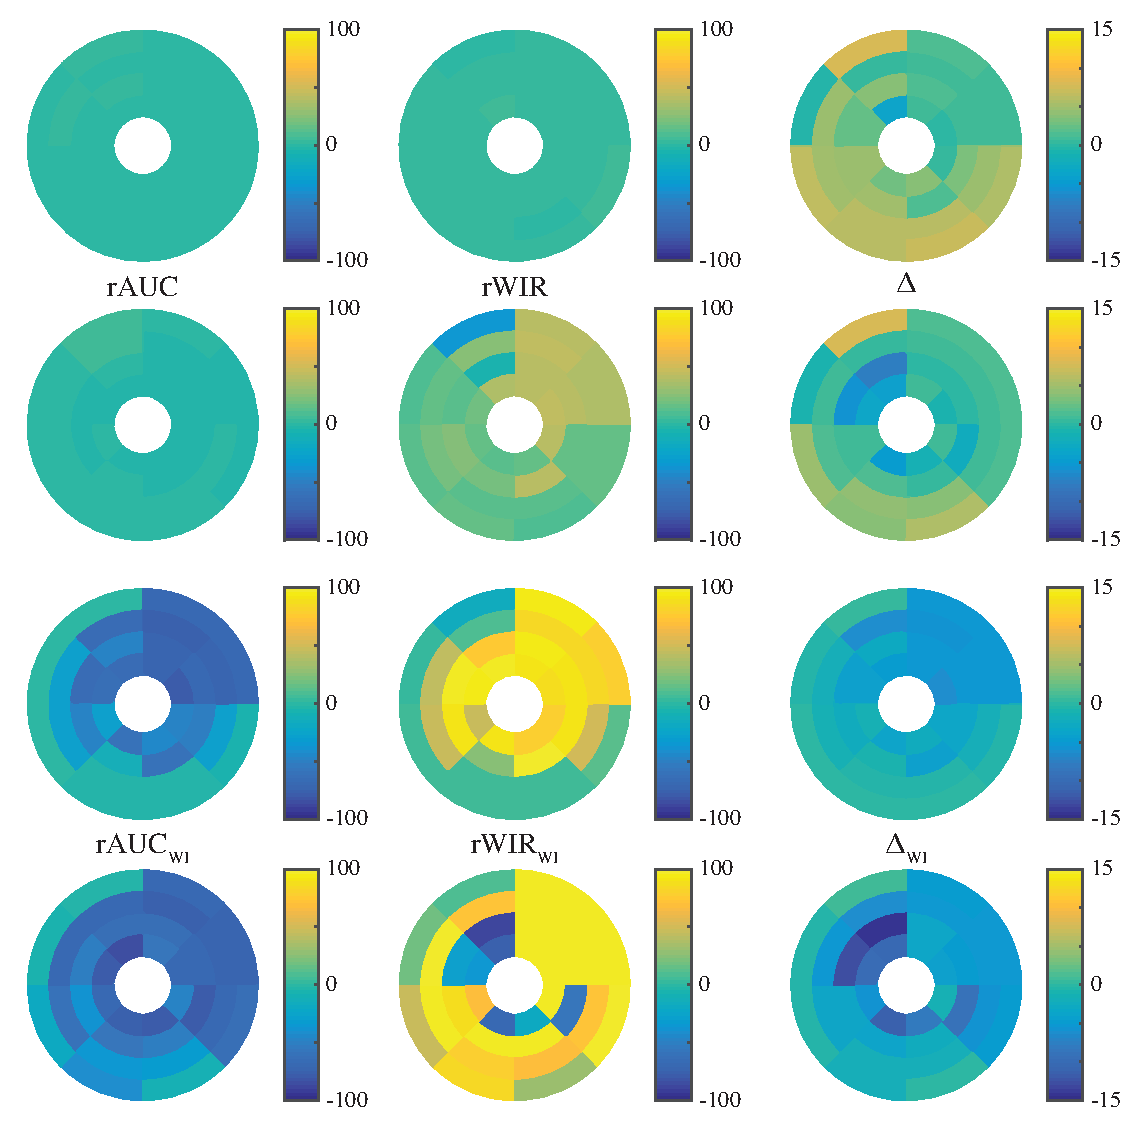
\includegraphics[width=\linewidth]{Ch5_simRC_bullseye_rLN_rLNwi.eps}
\caption{Bull's-eyes of the median estimation errors obtained by the rLN model at the intermediate noise level. From left to right: errors corresponding to tissue blood volume, tissue blood flow, time delay. From top to bottom: $M_3$ without recirculation, $M_3$ with recirculation, $M_4$ without recirculation, $M_4$ with recirculation.}
\label{fig:be-rLN}
\vspace{-3mm}
\end{figure}

\begin{figure}
\center
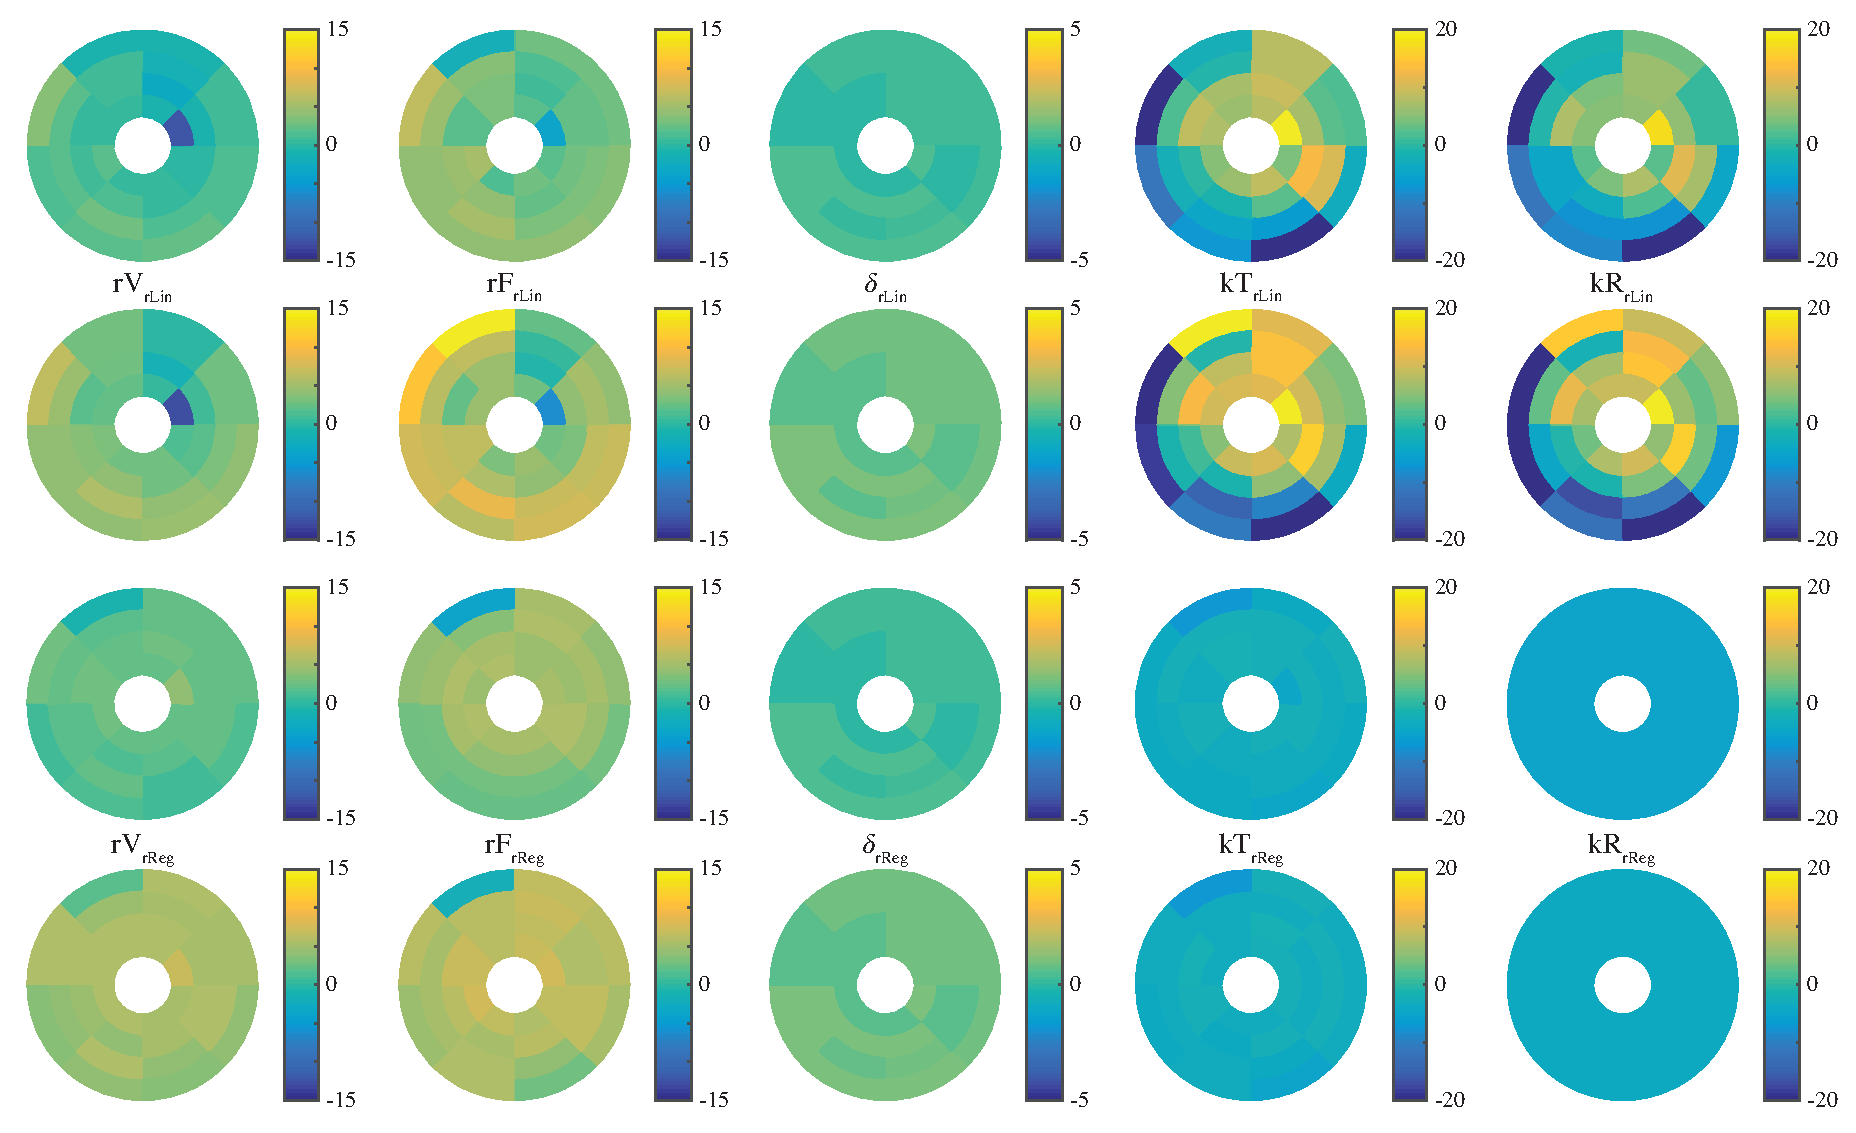
\includegraphics[width=\linewidth]{Ch5_simRC_bullseye_rLin_rReg.eps}
\vspace{-5mm}
\caption{Bull's-eyes of the median estimation errors obtained by the rLin and rReg models at the intermediate noise level. From left to right: errors corresponding to tissue blood volume, tissue blood flow, time delay, rate constant in tissue regions, rate constant in the reference tissue deduced from the different estimations inside tissue regions. From top to bottom: $M_5$ without recirculation, $M_5$ with recirculation, $M_6$ without recirculation, $M_6$ with recirculation.}
\label{fig:be-rLinReg}
\vspace{-3mm}
\end{figure}

\subsection{Model $M_1$}
When focusing on data without recirculation, the LN model (model $M_1$) is robust, it estimates accurate values of $AUC_i$ and $WIR_i$, whatever the level of noise. In particular, the intermediate noise level yields relevant estimates in all tissue regions. The time delay seems to be the less robust parameter but does not impact the reliability of the other parameters.
When introducing the recirculation model, the estimation of $AUC_i$ ($E \geq 25\%$), and in a less extent the estimation of $WIR_i$ ($E \leq 15\%$) are biased, but the bias does not vary with noise. As for the estimation of time-delays, behaviors similar to the LN model without recirculation can be observed.

\subsection{Model $M_2$}
When using the LN model restricted to the wash-in phase (model $M_2$), both $AUC_i$ and $WIR_i$ parameters are respectively largely under and over estimated, whatever the configuration, i.e.~without and with recirculation. Some disparities exist between regional parameters: the smallest values of tissue blood flow or tissue blood volume tend to provide larger relative estimation errors.

\subsection{Model $M_3$}
As expected, the rLN model (model $M_3$) for data without recirculation is robust, and provides accurate values of $rAUC_i$ and $rWIR_i$, whatever the level of noise and for the intermediate noise level, and the estimation is relevant in all regions. As could be anticipated, introducing recirculation, the estimation of $rAUC_i$ was rather accurate but the estimation of $rWIR_i$ was biased (bias invariant with noise), especially for smaller values of simulated tissue blood flow.

\subsection{Model $M_4$}
When using the rLN model restricted to the wash-in phase (model $M_4$), both $rAUC_i$ and $rWIR_i$ parameters were respectively largely under and over estimated, whatever the configuration: without and with recirculation. Results show similar trends to those observed when using the LN model restricted to the wash-in phase (model $M_2$).

\subsection{Model $M_5$}
The rLin model (model $M_5$) accurately estimates relative tissue blood volume and relative tissue blood flow parameters, exhibiting small biases, but the precision depends on the noise level. The estimation of time delays parameters appears to be robust. Biases are larger when taking into account studies with recirculation, but remain in most cases moderate ($E \leq 15\%$). Considering rate constants, some heterogeneity in estimated $k_R$ values was found. This confirms our assumption, since no constraints are applied to this specific values. Moreover, related errors appear in the estimates of $k_{T_i}$.

\subsection{Model $M_6$}
Compared with the model $M_5$, results using model $M_6$ are improved. By construction, a constant value of $k_R$ is estimated for all the subregions (slightly underestimated in the case shown in Figure~\ref{fig:be-rLinReg}), and consequently the relative error in the estimation of $k_{T_i}$ is highly homogeneous across tissue regions and almost constant. Indeed the largest median relative error on $k_{T_i}$ is observed for the highest value of simulated $k_{T_i}$. The rReg model estimates relative blood flow parameters and relative blood tissue parameters, with median relative errors generally less than 5\% without recirculation for the intermediate noise level (see Fig.~\ref{fig:be-rLinReg}). Of course, recirculation yields higher estimation errors, nevertheless they remain below 7\% in most cases and appear to be more homogeneous across the 32 subregions than the estimates of model $M_5$. 

\section{Discussion}
This study aimed at comparing the behavior of different models suitable for quantification of perfusion in contrast-enhanced ultrasound studies. Our whole analysis was based on simulated studies in order to have an irrefutable gold standard and to compare the different methods in terms of precision and accuracy. The model describing contrast displacement relies on a one-compartment model, that has proved to be valid to describe contrast enhancement in a murine tumor model~\cite{Doury2017wn}. In order to introduce some variations in the tissue blood flows, tissue blood volumes and time-delays, reflecting the regional heterogeneity among tissue regions, as observable with ultrasound. $N$ regions inside the simulated tissue of interest were introduced, each one being characterized by its set of perfusion parameters. In addition an arterial input function was first simulated using a single Log-Normal function, then approximated by a sum of modified Log-Normal functions to mimic recirculation. Although the deformation of the first-pass is quite simplistic, this approach enables us to consider two configurations: one idealized configuration without recirculation and one configuration closer to physiological conditions introducing recirculation. Finally different signal to noise conditions were simulated using a multiplicative noise model, as opposed to an additive Gaussian model, reflecting conditions encountered in contrast-enhanced ultrasound. Using 150 noisy simulations for each condition guarantees a representative set of possibilities, allowing generalization of the results, as well as enabling the study of the precision of the estimations.

The use of median and quartile operators to assess the estimation errors was necessary to reduce the impact of outliers, which were mostly found in the estimates of the rLin model. Using relative estimation errors (as opposed to absolute estimation errors) for tissue blood flows and tissue blood volumes related parameters allows easy comparison of the errors obtained for parameters with different simulated values. 

As expected, results of this study exhibit lower precision of the estimated parameters with decreasing signal to noise ratio. Interestingly, most of the methods are not strongly affected by the signal to noise ratio in terms of accuracy (reflected by the median error on parameters). In addition, perfusion parameters were found less accurate when estimated with recirculation, compared to the estimates without recirculation. 

The Log-Normal model, when applied to the whole duration of the study is robust to noise. However this model is subject to recirculation error. To get rid of this dependency, a naive approach consists in limiting the estimation of Log-Normal model to the first samples of the TIC (before recirculation occurs). However this solution appears to be unstable, providing estimates with huge discrepancies when compared to simulated parameters and also showing a large dependency to noise. This naive approach should therefore be absolutely avoided when dealing with dynamic perfusion data. Indeed results are not accurate for both configurations, i.e.~with or without recirculation. Thus the present simulation study also emphasizes the need for acquisitions with sufficiently long durations in order a reliably estimate perfusion parameters, and in particular when relying on the Log-Normal model for quantification. 

The use of a reference tissue to normalize perfusion parameters was already recommended following a test-retest study that was conducted on dynamic contrast-enhanced ultrasound acquisitions performed on small animals~\cite{Doury2017wn}. Normalization was also proposed by a clinical study in order to enable the comparison of perfusion parameters estimated using contrast-enhanced ultrasound data and contrast-enhanced computerized tomography~\cite{Lefort2012}. The present simulation study confirms the interest of normalization when looking at the accuracy and the precision of estimated parameters. Despite the use of the division operator that could be impacted by noise issues, normalized parameters are more accurate than ``absolute'' parameters when introducing recirculation in simulated TICs. As recirculation is physiological and cannot be suppressed experimentally, our results emphasis the need to address this question when dealing with real data.

Comparing the estimation of relative parameters using the rLN model, it appears that the $rAUC$ parameter is more precise than the $rWIR$ parameter. This experimental result is in concordance with the theory, as detailed in the appendix section of this paper. The differences which are observed between the estimated and simulated values of $rAUC$ in case of recirculation can partly be explained by the fitting of a Log-Normal model to the reference tissue prior to quantification. This step is useful to reduce the impact of noise but slightly inaccurate to represent TICs with recirculation, the use of a model-free noise-filtering technique should be investigated. To summarize it is important to note that in case of recirculation, the $rAUC$ is more representative of the simulated parameters than $AUC$.

The linear resolution of the relative one-compartment approach (method $M_5$) was introduced to process contrast-enhanced ultrasound studies in~\cite{Doury2016fi}. It ensures the fitting error reaches its global minimum, as opposed to the non-linear approach used in~\cite{Doury2017wn}. Furthermore, linear resolution significantly reduces computing-time. Some aberrant values of perfusion parameters can however be found since parameters were not bounded during the estimation process. As indicated in the theory section, applying this method independently to multiple regions yields multiple values of $k_R$, this effect was also shown in Figure~\ref{fig:estpar4} and Figure~\ref{fig:be-rLinReg}. Method $M_6$ simply enforces a single value of $k_R$ should be estimated across tissue regions. As a consequence, the approach yields spatially regularized estimates of $k_T$, slightly biased. As expected, the impact of recirculation on estimates of models $M_5$ and $M_6$ is rather low, however not negligible. This effect could be partly explained by the approximation of the TIC inside the reference tissue by the Log-Normal model which does not account for recirculation. This prior modeling was performed in order to reduce the impact of noise on the relative perfusion parameters.
The median relative errors on these parameters are all less than 7\%, even in presence of recirculation, which acceptable. This is illustrated in Figure~\ref{fig:be-rLinReg} for an intermediate noise level. 

The estimation of absolute values of perfusion parameters is possible, at least theoretically. It would however require an accurate estimation of the arterial input function. Its proper estimation from image data is a large research question which is not fully solved, even considering other perfusion imaging modalities such as MRI or PET. Some problems are inherent to ultrasound data, ranging from the calibration of signal intensity according to the amount of injected contrast agent, to issues resulting from the 2D nature of data. Additionally, the estimation of such a function in small vessels, surrounding a tumor for instance, is subject to partial volume effects, along with small displacements effects. Therefore, when quantifying CEUS data, we recommend using relative parameters, i.e.~parameters normalized according to a reference tissue. Indeed, the chosen reference tissue should be accessible and rather homogeneous. However the robustness of the rLin and rReg models to the choice of the reference tissue remains to be fully investigated.
 
\section{Conclusion}
This study was designed to investigate the impact of recirculation on the quantification of contrast-enhanced ultrasound exams, by means of simulations based on experimental data. 
Fitting a Log-Normal model on the first pass of the bolus implies a reduction of the number of points used to fit the model and yields unstable estimates, especially on noisy data. This solution is thus inappropriate. Modeling methods such as compartmental modeling, that account for recirculation intrinsically, are indeed the most robust to recirculation. Making use of a reference tissue, the estimation of relative parameters appears to be robust. Taking advantage of the multiple regions, and enforcing estimation of a single rate constant characterizing the reference tissue, provides stable estimates, especially when comparing parameter estimates across regions. This approach is therefore recommended because of its reduced sensitivity to recirculation, and better homogeneity of the estimates inside the considered field of view. 

\section*{Appendix}
Taking into account the generic expression of the Log-Normal model:
\begin{equation*}
\frac{A}{\sqrt{2 \pi}\sigma (t- \tau)} \exp \left( - \frac{\left[ \ln{(t- \tau)} - \mu \right]^2}{2{\sigma}^2} \right)
\end{equation*}
and considering the formal definitions of the area under the curve and of the wash-in rate, it can be deduced:
\begin{eqnarray*}
AUC &= & A \\
WIR &= &\frac{A}{\sigma\sqrt{2\pi}}\left(\frac{y}{\sigma^2}-1\right)e^{2y-2\mu-\frac{y^2}{2\sigma^2}} \\
%\text{with}
\text{with} \quad y &= &\frac{3\sigma^2+\sigma\sqrt{\sigma^2+4}}{2}
\end{eqnarray*}
These equations were directly used to compute the $AUC$ and $WIR$ parameters from a Log-Normal approximation.

$AUC$ and $WIR$ can also be derived when considering a one-compartment vascular model, their expression is computed for two cases in the following table: one simplified case assuming that $C_A(t)$ follows a gate function and the general case. In addition relative parameters $rAUC$ and $rWIR$ are formally computed when considering a reference tissue. 
Using the gate function for $C_A(t)$ shows a strong equivalence between $AUC$ and tissue blood volume $V$, but also between $WIR$ and tissue blood flow $F$. Thus, for that case, $rAUC = rV$ and $rWIR = rF$. 
Using the general shape for $C_A(t)$ shows that $AUC$ is strictly proportional to $V$, and that $rAUC = rV$. Furthermore, $WIR$ is related to $F$, but $rWIR$ is not strictly identical to $rF$, since a corrective factor $\rho$ is introduced. This factor depends of the time of inflexion (denoted $t_I$) of each TIC and explains why the $rWIR$ is generally not strictly equivalent to $rF$.

\begin{table}[h!]
\begin{center}
\begin{tabular}{lcc}
\toprule
AIF & $K rect_a\left(t\right)$ & $C_A \left(t\right)$ \\
\midrule
\textbf{$AUC$} & $KV_T$ & $V_T \int_{0}^{+\infty}C_A\left(\tau\right)\mathrm d\tau$\\
\midrule
\multirow{3}{*}{\textbf{$WIR$}}
 & \multirow{3}{*}{{$\frac{KF_T}{a}$}} & $F_T\left(C_A\left(t_{I}\right)-\frac{1}{V_T}C_T\left(t_{I} - D_T\right)\right)$ \\
 & & $\{ t_{I} \enskip\vert\enskip \frac{\mathrm d C_T}{\mathrm dt}\left(t_{I} - D_T\right) = V_T \frac{\mathrm d C_A}{\mathrm dt}\left(t_{I}\right),$ \\
 & & $\frac{\mathrm d C_A}{\mathrm d t}\left(t_{I}\right) > 0\}$ \\
\midrule
\textbf{$rAUC$} & $rV$ & $rV$\\
\midrule
\textbf{$rWIR$} & $rF$ & $\rho \cdot rF$\\
\bottomrule
\end{tabular}
\caption{Analytic expressions of perfusion parameters using a one-compartment model and assuming two different shapes of AIF: rectangle function of width $a$ and height $1/a$, $rect_a(t)$, and general case $C_A(t)$. In the first case, $K$ stands for the injected concentration.}
\label{tab:AppAnalyticRelationAIF}
\end{center}
\end{table}

\bibliographystyle{plainnat}
\bibliography{Bibliography/chap5}